\documentclass[11pt]{article}

\usepackage[margin=1in]{geometry}
\usepackage{graphicx}
\usepackage{float}
\usepackage{amsmath}
\usepackage{amssymb}
\usepackage{booktabs}
\usepackage{subcaption}
\usepackage{hyperref}
\usepackage{xcolor}

\hypersetup{
    colorlinks=true,
    linkcolor=blue,
    urlcolor=blue,
    citecolor=blue
}

\title{EE443 Homework 4\\
Diffusion Models and Vision Transformer Classification}
\author{Rishabh Goenka}
\date{Spring 2026}

\begin{document}

\maketitle
\tableofcontents
\newpage

% =====================================================
\section{Problem 1: Diffusion Models (30\%)}

\subsection{1-(a) Toy Dataset Diffusion}

\subsubsection*{1) Purpose of the noise prediction model}

In diffusion training, the model learns to predict the Gaussian noise that was added to a clean sample at a randomly selected time step. This lets the model learn the reverse denoising process. During generation, the model starts from random noise and repeatedly removes predicted noise to produce samples from the target data distribution.

\subsubsection*{2) Final training loss and test loss}

\[
\text{Final Test Loss} = 0.4086
\]

From the Q1 training curve endpoint, the final training loss is approximately in the low-$0.3$ range (slightly below the final test loss).

\subsubsection*{3) Generated 2D samples using different numbers of sampling steps}

\begin{figure}[H]
    \centering
    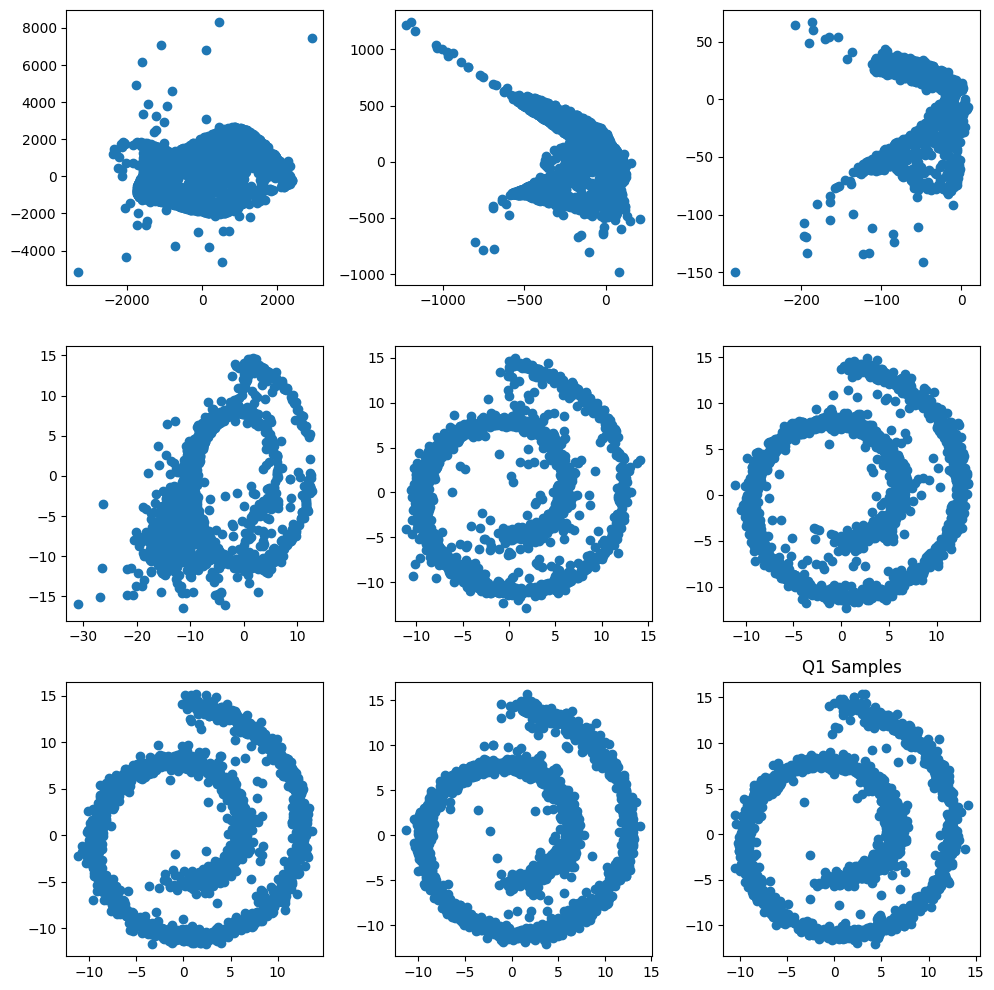
\includegraphics[width=0.9\textwidth]{figures/q1_samples_steps.png}
    \caption{Generated toy 2D samples for different diffusion sampling step counts.}
\end{figure}

\subsubsection*{4) Effect of sampling-step count on quality}

With very few reverse steps, samples are generally noisier and less aligned with the target manifold. As the number of sampling steps increases, denoising is more gradual and the generated distribution better matches the data geometry. After a point, quality gains become smaller while runtime keeps increasing.

\begin{figure}[H]
    \centering
    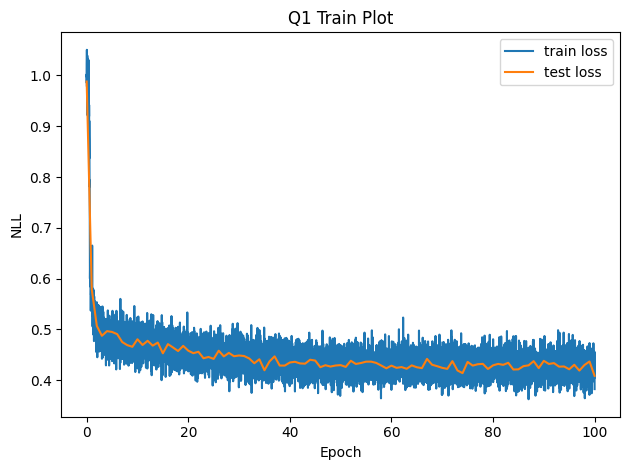
\includegraphics[width=0.72\textwidth]{figures/q1_train_curve.png}
    \caption{Q1 training and validation loss curve.}
\end{figure}

% -----------------------------------------------------
\subsection{1-(b) Pixel-Space Diffusion on CIFAR-10}

\subsubsection*{1) Final training loss and test loss}

\[
\text{Final Test Loss} = 0.0618
\]

From the Q2 training curve endpoint, the final training loss is approximately in the low-$0.05$ range.

\subsubsection*{2) Representative generated CIFAR-10 images}

\begin{figure}[H]
    \centering
    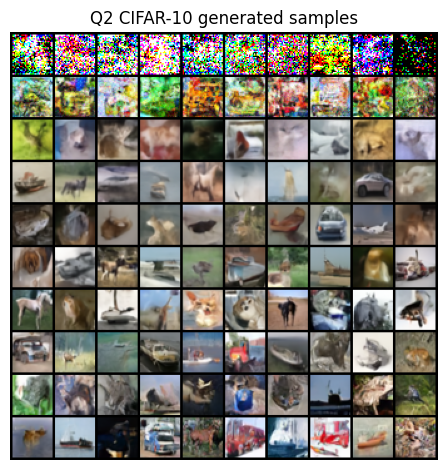
\includegraphics[width=0.95\textwidth]{figures/q2_cifar_samples_steps.png}
    \caption{Generated CIFAR-10 images across different numbers of diffusion sampling steps.}
\end{figure}

\subsubsection*{3) Comparison across sampling-step counts}

At low step counts, generated images tend to be blurrier and less semantically consistent. Increasing the number of steps improves structure and texture because each denoising update is less aggressive. Very large step counts still improve quality but with diminishing returns relative to additional computation.

\subsubsection*{4) One limitation of pixel-space diffusion vs latent-space diffusion}

Pixel-space diffusion operates directly on high-dimensional image tensors, so training and sampling are expensive in memory and compute. Latent-space diffusion denoises in a compressed representation, which is typically faster and more efficient.

\begin{figure}[H]
    \centering
    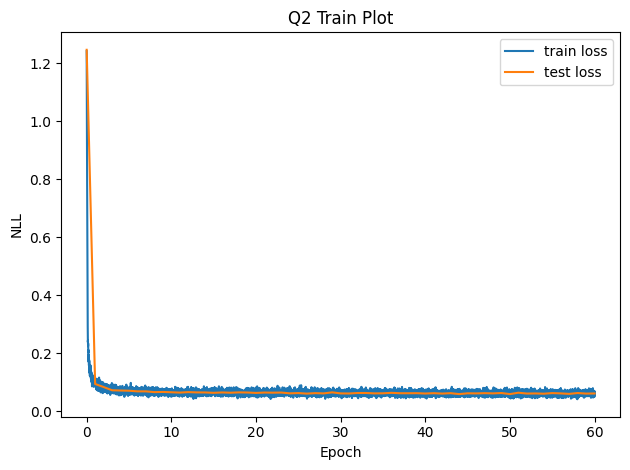
\includegraphics[width=0.72\textwidth]{figures/q2_train_curve.png}
    \caption{Q2 training and validation loss curve.}
\end{figure}

% -----------------------------------------------------
\subsection{1-(c) Class-Conditional Latent-Space Diffusion with DiT}

\subsubsection*{1-(c-i) VAE reconstructions and latent scale factor}

\textbf{(1) Original and reconstructed CIFAR-10 examples}

\begin{figure}[H]
    \centering
    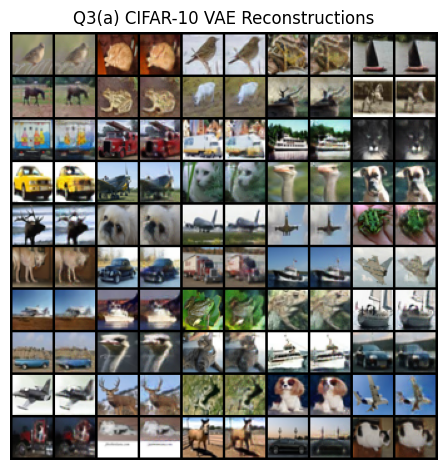
\includegraphics[width=0.95\textwidth]{figures/q3a_vae_reconstructions.png}
    \caption{Original CIFAR-10 images and corresponding VAE reconstructions.}
\end{figure}

\textbf{(2) Estimated latent scale factor}

\[
\text{Scale Factor} = 1.2479
\]

\subsubsection*{1-(c-ii) Class-conditional DiT training}

\textbf{(3) Final training loss and test loss for latent diffusion}

\[
\text{Final Test Loss} = 0.3571
\]

From the Q3(b) training curve endpoint, the final training loss is approximately in the low-$0.3$ range.

\textbf{(4) Generated class-conditional samples}

\begin{figure}[H]
    \centering
    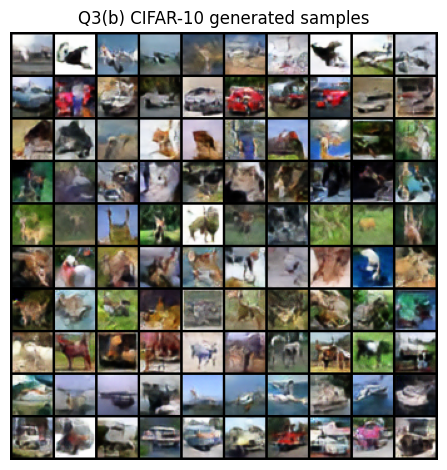
\includegraphics[width=0.95\textwidth]{figures/q3b_class_conditional_samples.png}
    \caption{Class-conditional generated samples from the DiT latent diffusion model.}
\end{figure}

\begin{figure}[H]
    \centering
    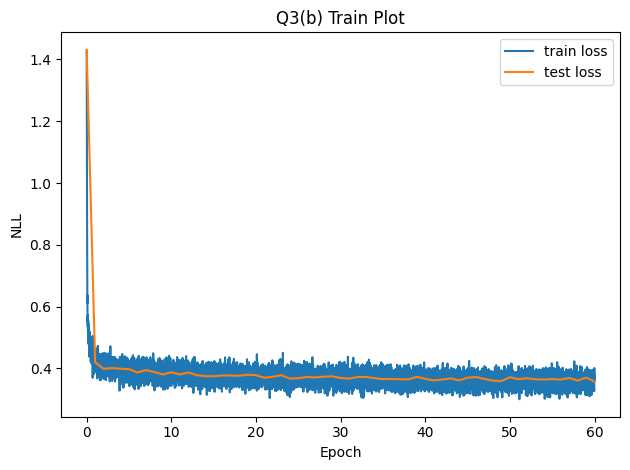
\includegraphics[width=0.72\textwidth]{figures/q3b_train_curve.png}
    \caption{Q3(b) training and validation loss curve.}
\end{figure}

\subsubsection*{1-(c-iii) Classifier-free guidance (CFG)}

\textbf{(5) Samples for different CFG strengths}

\begin{figure}[H]
    \centering
    \begin{subfigure}{0.48\textwidth}
        \centering
        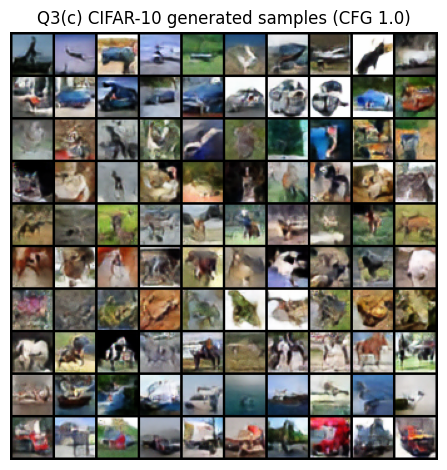
\includegraphics[width=\textwidth]{figures/q3c_cfg_w1_0.png}
        \caption{$w = 1.0$}
    \end{subfigure}
    \hfill
    \begin{subfigure}{0.48\textwidth}
        \centering
        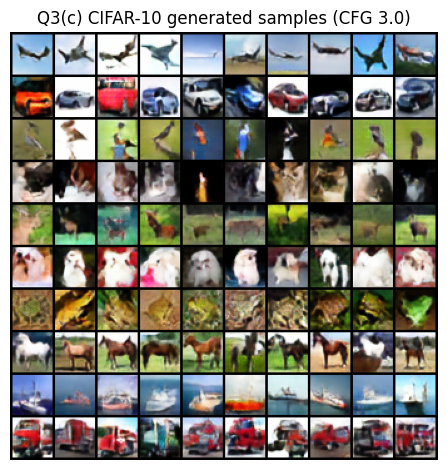
\includegraphics[width=\textwidth]{figures/q3c_cfg_w3_0.png}
        \caption{$w = 3.0$}
    \end{subfigure}
    \vspace{0.6em}
    \begin{subfigure}{0.48\textwidth}
        \centering
        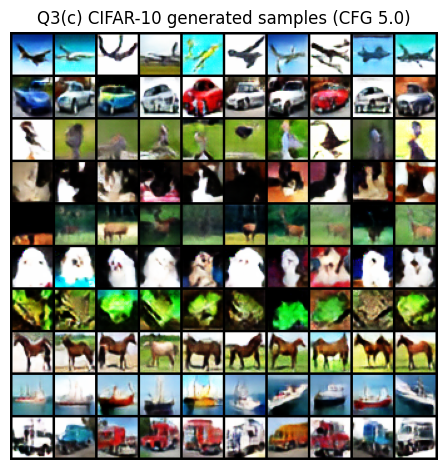
\includegraphics[width=\textwidth]{figures/q3c_cfg_w5_0.png}
        \caption{$w = 5.0$}
    \end{subfigure}
    \hfill
    \begin{subfigure}{0.48\textwidth}
        \centering
        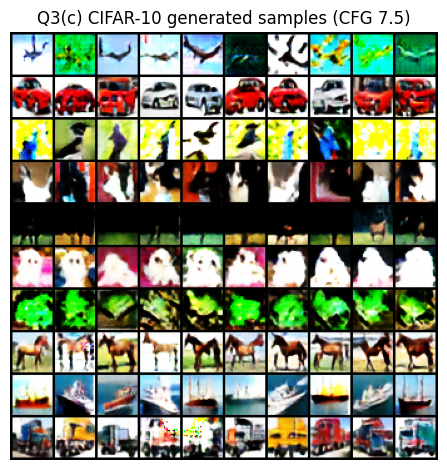
\includegraphics[width=\textwidth]{figures/q3c_cfg_w7_5.png}
        \caption{$w = 7.5$}
    \end{subfigure}
    \caption{Classifier-free guidance outputs for multiple guidance strengths.}
\end{figure}

\textbf{(6) How CFG changes generation; too small vs too large guidance}

Increasing CFG generally improves class alignment up to a moderate range, because conditional information is emphasized more strongly. If guidance is too small, samples can look less class-specific and more generic. If guidance is too large, samples may become over-sharpened, oversaturated, or less diverse due to over-amplification of the conditional direction.

% =====================================================
\section{Problem 2: Vision Transformer Image Classification (30\%)}

\subsection{2-(a) Dataset Inspection and Preprocessing}

\textbf{1) Number of training examples, test examples, and Food-101 classes}

\begin{itemize}
    \item Training examples: \textbf{4000}
    \item Test examples: \textbf{1000}
    \item Number of classes: \textbf{101}
\end{itemize}

\textbf{2) Example training images and labels}

\begin{figure}[H]
    \centering
    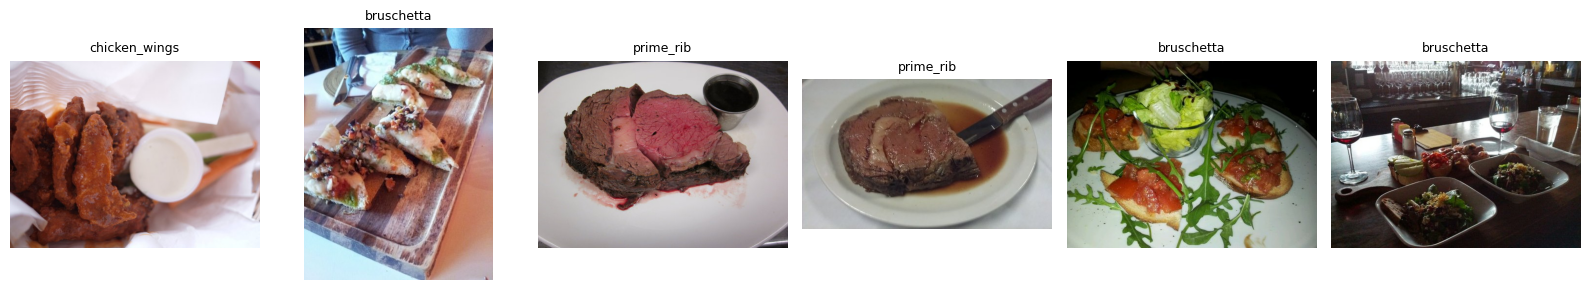
\includegraphics[width=0.95\textwidth]{figures/q2a_training_examples.png}
    \caption{Training-split Food-101 examples with labels.}
\end{figure}

\textbf{3) Why resize/crop and normalize before ViT}

The pretrained ViT expects fixed-size inputs (224x224 here) and a specific pixel distribution. Resize/crop ensures the patch embedding layer receives the right spatial dimensions, and normalization matches the statistics used during pretraining. This keeps feature activations in the expected range and improves transfer performance.

\textbf{4) What goes wrong if normalization stats do not match}

If input mean/std are mismatched, the model sees shifted/scaled inputs compared to pretraining. This can degrade calibration and class separation, causing lower accuracy and less stable optimization.

% -----------------------------------------------------
\subsection{2-(b) Metric Computation and ViT Model Setup}

\textbf{1) How predicted class is obtained from logits}

The model outputs one logit per class. The predicted class is the index of the largest logit:
\[
\hat{y} = \arg\max_k \text{logits}_k.
\]

\textbf{2) Is accuracy always sufficient?}

Not always. For imbalanced class distributions, a model can achieve high overall accuracy by performing well on frequent classes while still failing on rare classes. In that case, class-wise precision/recall or macro-F1 is more informative.

\textbf{3) Which part is pretrained vs newly initialized}

The ViT backbone (patch embeddings + transformer encoder layers) is loaded from the pretrained checkpoint. The final classifier layer is adapted for 101 Food-101 classes and is newly initialized for this task.

\textbf{4) Why ViT splits images into patches}

Self-attention operates on token sequences. ViT converts the image into a sequence of patch tokens so global attention can model long-range relationships across the full image.

% -----------------------------------------------------
\subsection{2-(c) Fine-Tuning and Evaluation}

\textbf{1) Final validation accuracy and evaluation loss}

\[
\text{Final Validation Accuracy} = 0.953
\]
\[
\text{Final Evaluation Loss} = 0.42274072766304016
\]

\textbf{2) Main training settings}

\begin{itemize}
    \item Learning rate: \texttt{5e-5}
    \item Train batch size: \texttt{16}
    \item Eval batch size: \texttt{16}
    \item Number of epochs: \texttt{3}
\end{itemize}

\textbf{3) Effect of increasing batch size, learning rate, or epochs}

Larger batch sizes generally improve throughput but increase memory usage and can reduce generalization if too large. Larger learning rates can speed up early optimization but may destabilize training if excessive. More epochs can improve fit up to a point, then increase overfitting risk.

\textbf{4) One ViT strength vs one CNN strength}

A ViT strength is global context modeling via attention across distant regions. A CNN strength is strong local inductive bias (translation-equivariant filters), which often makes CNNs more data-efficient on smaller datasets.

% -----------------------------------------------------
\subsection{2-(d) Inference and Error Analysis}

\textbf{1) Validation figure with predicted and true labels}

\begin{figure}[H]
    \centering
    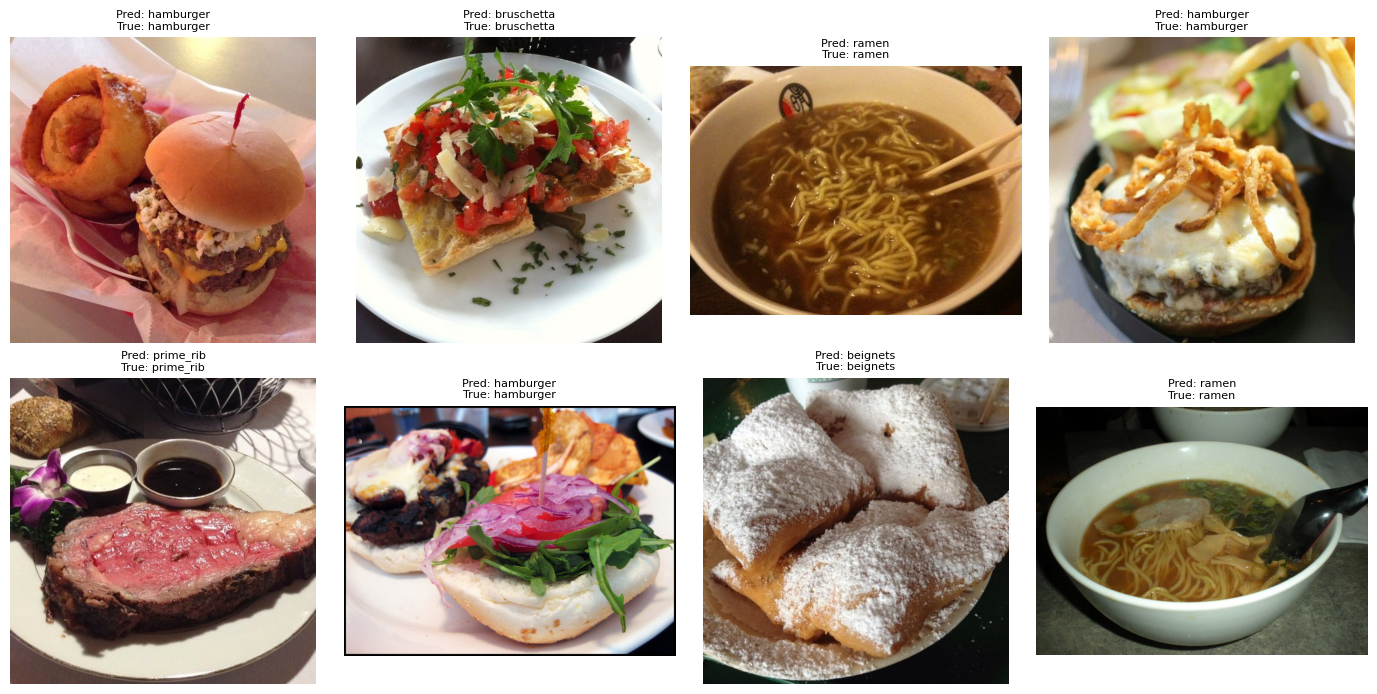
\includegraphics[width=0.95\textwidth]{figures/q2d_validation_predictions.png}
    \caption{Validation examples with predicted and true labels.}
\end{figure}

\textbf{2) At least two correct and two incorrect predictions}

The figure includes multiple correct predictions where predicted and true labels match. For incorrect predictions, the notebook's explicit error scan among the first 100 validation examples reported:
\begin{itemize}
    \item \texttt{index=23 | pred=pork\_chop | true=prime\_rib}
    \item \texttt{index=74 | pred=beignets | true=prime\_rib}
\end{itemize}

\textbf{3) Why examples may be classified correctly or incorrectly}

Correct predictions are typically cases where class-specific visual cues (shape, texture, plating style) are clear after preprocessing. The mistakes above are plausible because meat-based classes can be visually similar, and crop/scale changes can remove context needed for disambiguation.

\textbf{4) One limitation of this experiment}

The experiment used a reduced subset and a short training schedule (3 epochs), which may limit robustness to intra-class variation and edge cases despite strong validation accuracy.

\end{document}

